\chapter{模糊最大熵模型分类应用研究}

\section{IRIS数据集}
\par
此数据是来自UCI的鸢尾花(iris)数据集.
这是一个经典的分类数据集,由Iris Setosa(山鸢尾)、Iris Versicolour(杂色鸢尾)和Iris Virginica(维吉尼亚鸢尾)三种不同类别的鸢尾花组成,
每个样本由四个属性组成,分别是Petal.Length(花瓣长度)、Petal.Width(花瓣宽度)、Sepal.Length(花萼长度)和Sepal.Width(花萼宽度).
按两两属性绘制原始数据如下:
\begin{figure}[!ht]
    \centering
    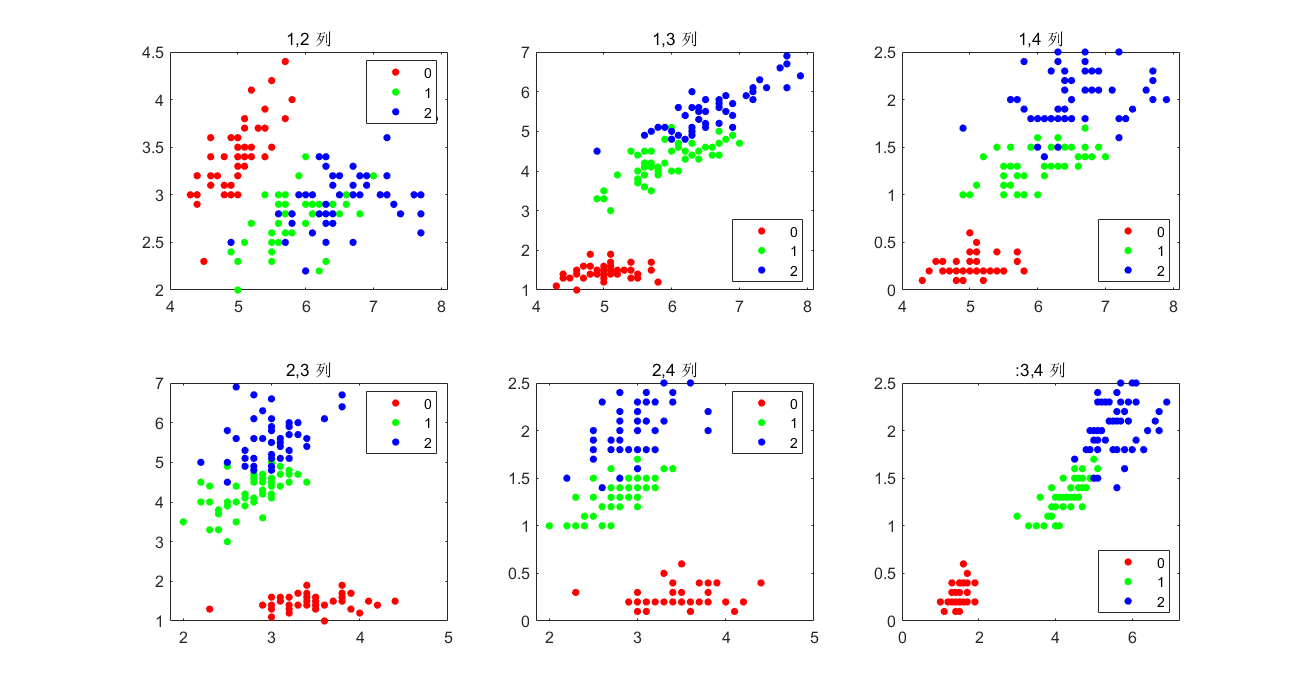
\includegraphics[scale=0.4]{sandiantu.png}
    \caption{原始数据散点图}
    \label{散点图}
\end{figure}
\par 按4.1的算法对iris数据集进行聚类,结果如下:
\begin{table}[!ht]
    \label{聚类中心}
    \caption{聚类中心}
    \centering
    \begin{tabular}{c c c c c}
        \whline & sepal length & sepal width & petal length & petal width \\\whline
        $v_1$   & 5.0136       & 3.3903      & 1.5369       & 0.2781      \\
        $v_2$   & 6.4737       & 2.9437      & 5.1910       & 1.8012      \\
        $v_3$   & 6.0922       & 2.8186      & 4.6775       & 1.5731      \\
        \whline
    \end{tabular}
\end{table}
\begin{figure}[!ht]
    \centering
    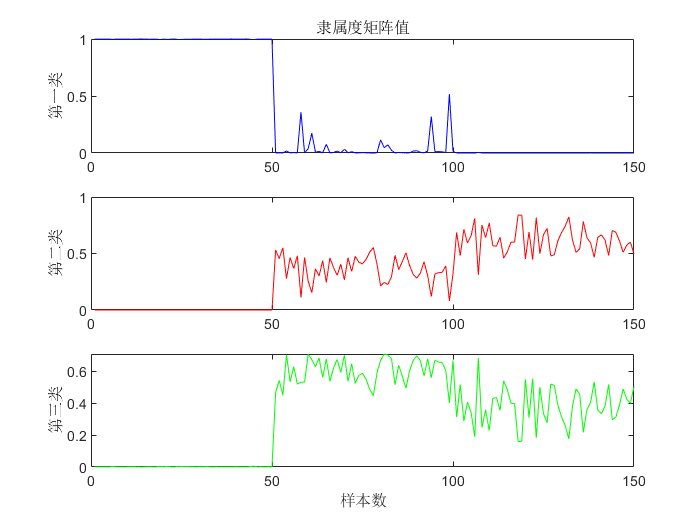
\includegraphics[scale=0.6]{lishudu.png}
    \caption{隶属度矩阵的值}
    \label{隶属度}
\end{figure}
\newpage
与FCM算法分类结果比较
\begin{table}[!ht]
    \label{准确率比较}
    \caption{准确率比较}
    \centering
    \begin{tabular}{c | c c c c}
        \whline 算法/各类准确率 & Setosa(山鸢尾) & Versicolour(杂色鸢尾) & Virginica(维吉尼亚鸢尾) & 总样本 \\\whline
        K-means                & 100\%          & 96\%                  & 72\%                    & 89.4\%   \\
        FCM                    & 100\%          & 76\%                  & 94\%                    & 90\%   \\
        MFE                    & 100\%          & 86\%                  & 98\%                    & 94.7\% \\
        \whline
    \end{tabular}
\end{table}
从数据的比较中,可以看到,对于第一类,三个算法都做到了很好的识别,但是对于后两类非线性相关的类别,模糊最大熵模型比其他两个模型有着更好的表现.
\section{红酒数据集}

